%!TEX root = ../dokumentation.tex
\lstset{
	frame=single,
	keywordstyle=\color{blue},
	commentstyle=\color{green},
	numbers=left,
}

\chapter{Backend}

\section{Programmarchitektur}
\todo{UML}


\section{Serverseite}
\begin{lstlisting}[caption={Serverseitige Implementierung für das Anwenden der Hilfestellungen}, label={lst:Serverseitig}]
	@socketio.on('help')
	def help():
	global help_step
	global technique_result
	errors = sudoku.get_errors()
	if errors:
	print(errors)
	emit('showErrors', errors)
	return
	if help_step == 0:
	sudoku.update_candidates()
	technique_result = technique_manager.try_techniques(sudoku.board, sudoku.candidates)
	if not technique_result:
	print("No suitable technique found!")
	return
	emit('help0',
	{'name': technique_result['name'], 'primaryCells': technique_result['primary_cells'],
		'secondaryCells': technique_result['secondary_cells']})
	elif help_step == 1:
	candidates()
	emit('help1', {'highlights': technique_result['highlights'], 'crossOuts': technique_result['cross_outs']})
	elif help_step == 2:
	emit('help2', {'name': technique_result['name'], 'explanation': technique_result['explanation']})
	elif help_step == 3:
	if technique_result['name'] in ['Naked Single', 'Hidden Single', 'Third Eye']:
	data = {'number': technique_result['highlights'][0]['value'],
		'checkedCells': [technique_result['highlights'][0]['cell']]}
	emit('help3')
	new_numbers(data)
	help_step -= 1
	else:
	sudoku.remove_candidates(technique_result['cross_outs'])
	candidates()
	emit('help3')
	help_step += 1
	help_step %= 4
\end{lstlisting}

\section{SudokuBoard}
\subsection{Datenstruktur des Sudokuboards}
\begin{figure}[htbp]
	\centering
	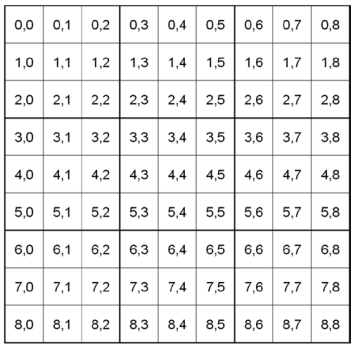
\includegraphics[width=0.3\textwidth]{images/board.png}
	\caption{Struktur des Sudokuboards und Zellenidentifikation}
	\label{fig:Sudokugitter}
\end{figure}

\subsection{Funktionalität}



\section{Technique Manager}
\todo{Reihenfolge der Techniken nach einfach zu schwer, tequniqe ist ein Liste von Klassenrepräsentationen umgesetzter Techniken}
In der Datei \textit{technique\_manager.py} wird das Aufrufen der Techniken geregelt. Die Techniken sind in einer Liste gespeichert. Über diese Liste wird drüber iteriert und das Board und die Kandidaten übergeben. Danach wird die abstrakte Methode \textit{execute\_technique()} für die Lösungstechnik ausgeführt. Der Returnwert dieser Methode ist True, wenn sich etwas an dem Board oder an den Kandidaten verändert. In diesem Fall wird die Methode \textit{get\_result()} aufgerufen, mit der die Änderungen durchgeführt werden können.
Wenn eine Technik nicht erfolgreich ist dann wird mit der nächsten Lösungsstrategie aus der Liste weiter gemacht. 

\begin{lstlisting}[language=Python, caption={Funktion um eine anwendbare Lösungstechnik zu finden}, label={lst:try}]
	def try_techniques(board, candidates):
		for tech in techniques:
			technique = tech(board, candidates)
			successful = technique.execute_technique()
			if successful:
				return technique.get_result()
		return False
\end{lstlisting}

\section{Abstrakte Klasse SolvingTechniques}
\todo{Möglichmacher für Liste der Klassen, daher können alle auf selbe Art und weise instanziiert werden und gleiche funktionen.}

\subsection{Abstrakte Methoden}

\subsubsection{configure\_highlighting(self)}
\subsubsection{execute\_technique(self)}
\subsubsection{update\_explanation(self)}

\subsection{Hilfsfunktionen}
\todo{es gibt in der abstrakten Methode berits implementierte Hilfsfunktionen, Nutzung bei mehreren Lösungstechniken notwenidg/hilfreich}

\section{Lösungsstrategien}

In diesem Abschnitt wird ein Überblick über die implementierten Strategien gegeben. Die Lösungsstrategien sind auf der Website \url{https://www.thinkgym.de/rätselarten/sudoku/} betitelt und beschrieben. Anhand diesen Beschreibungen wurden einige Lösungsstrategien implementiert. Zunächst wird ein Überblick über die umgesetzten Strategien gegeben, bevor ausblickend die Lösungsstrategien, die noch nicht implementiert wurden, aufgezählt werden. Es gibt noch weitere Strategien die auf der Website nicht beschrieben werden. Diese werden im Folgenden aber nicht weiter beachtet.

\subsection{Umgesetzte Lösungsstrategien}
Da in der Ausarbeitung nur exemplarisch auf einige Lösungsstrategien eingegangen wird, wird hier aufgezählt welche Strategien alle umgesetzt wurden. 
\begin{itemize}
	\item Versteckter Single (Hidden Single)
	\item Nackter Single (Naked Single)
	\item Nacktes Paar (Naked Pair)
	\item Verstecktes Paar (Hidden Pair)
	\item Nackter Dreier (Naked Triple)
	\item Versteckter Dreier (Hidden Triple)
	\item Nackter Vierer (Naked Foursome)
	\item Versteckter Vierer (Hidden Foursome)
	\item \acf{RBC} (Line-Block-Interaction)
	\item \acf{BRC} (Block-Line-Interaction)
	\item X-Wing (X-Wing)
	\item Steinbutt (Turbot)
	\item Drittes Auge (Third Eye)
	\item Wolkenkratzer (Skyscraper)
	\item Schwertfisch (Swordfish)
	\item Drachen (Dragon)
	\item Verbotenes Rechteck Typ 1 (Forbidden Rectangle Type 1)
	\item Verbotenes Rechteck Typ 2 (Forbidden Rectangle Type 2)
	\item Verbotenes Rechteck Typ 4 (Forbidden Rectangle Type 4)
	
\end{itemize}

\subsection{Weitere Lösungsstrategien}
In der Studienarbeit wurden nicht alle auf der Website \cite{martin} vorgestellten Lösungstechniken umgesetzt. Weitere Strategien die noch implementiert werden könnten sind die folgenden:
\begin{itemize}
	\item Erweiterter \ac{BRC}
	\item (noch nicht) Verbotenes Rechteck Typ 3
	\item (noch nicht) XY-Wing
	\item (noch nicht) XYZ-Wing
	\item (noch nicht) X-Kette
	\item (noch nicht) XY-Kette
	\item (noch nicht) Schwertfisch mit Flosse
	\item (noch nicht) W-Wing
	\item (noch nicht) Geklonte Paare
	\item (noch nicht) Leeres Rechteck
	\item (noch nicht) Doppelkette
	\item (noch nicht) Forcing Chain
\end{itemize}
Der Erweiterte \ac{BRC} wurde nicht umgesetzt, weil es eine Kombination aus dem \ac{BRC} und einem Versteckten Single ist. 

\section{Beispielhafte Umsetzung von Strategien}
Die Lösungsstrategien können zwei unterschiedliche Wirkungen auf ein Sudokurätsel haben. Entweder es ist möglich eine Zahl einzufügen oder es können Kandidaten aus verschiedenen Gründen eliminiert werden. Diese beiden Wirkungen werden im Backend unterschiedlich behandelt. In den nächsten zwei Unterkapiteln wird die Funktionsweise und die Unterschiede beider Varianten anhand zweier Beispiele erklärt. 

Für beide Umsetzungen wird die Abstrakte Klasse \textit{SolvingTechniques} genutzt.

\subsection{Zahl einfügen}

Der Fall, dass aufgrund einer Lösungstechnik direkt eine Zahl in das Sudokugitter eingetragen werden kann, gibt es nur bei drei Techniken. Für alle anderen Techniken ist das eintragen einer Zahl maximal das Resultat von dem Herausstreichen einer Zahl. 
\begin{itemize}
	\item Versteckter Single
	\item Nackter Single
	\item Drittes Auge
\end{itemize}

\subsection{Kandidat eliminieren}
